\begin{figure}[!ht]  
  % \vspace{-0.2cm}
  \centering
  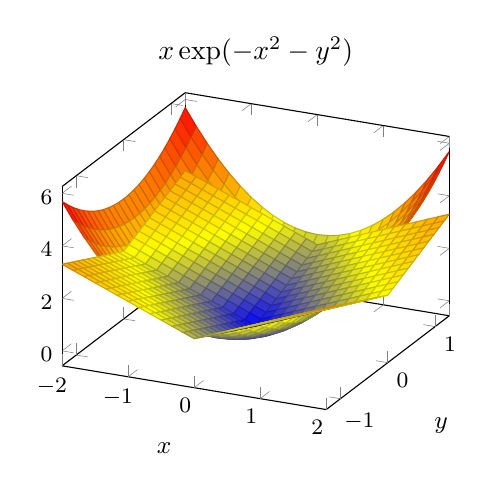
\begin{tikzpicture}
    \begin{axis}[
      title={$x \exp(-x^2-y^2)$},
      xlabel=$x$, ylabel=$y$,
      small,
      ]
      \addplot3[
      surf,
      domain=-2:2,
      domain y=-1.3:1.3,
      ]
      {x^2+y^2};

      \addplot3[
      surf,
      domain=-2:2,
      domain y=-1.3:1.3,
      ]
      {(x^2)^0.5+(y^2)^0.5};

    \end{axis}
  \end{tikzpicture}

  % \begin{tikzpicture}
  %   \begin{axis}[
  %     title={$x \exp(-x^2-y^2)$},
  %     enlarge x limits,
  %     view={0}{90},
  %     xlabel=$x$, ylabel=$y$,
  %     small,
  %     ]
  %     \addplot3[
  %     domain=-2:2,
  %     domain y=-1.3:1.3,
  %     contour gnuplot={number=14},
  %     thick,
  %     ]
  %     {x^2+y^2};
  %   \end{axis}
  % \end{tikzpicture}
  % \includegraphics[height=6cm]{images/alpha_vec/testing.png}
  \caption{Plot of $h_\alpha(x)$ for various values of $\alpha$.}  
  \label{fig:power_norm}
\end{figure}


%%% Local Variables:
%%% mode: latex
%%% TeX-master: "../main"
%%% End:
